\begin{frame}{Trigonometrie}
	\begin{columns}
	\column{.6\textwidth}
	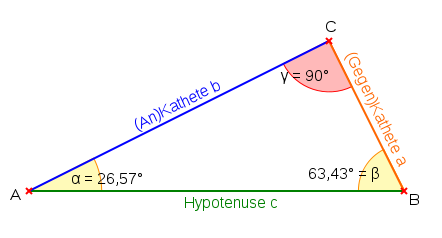
\includegraphics[width=1.1\textwidth,height=.8\textheight,keepaspectratio]{dreieck.png}
	\column{.4\textwidth}
	\begin{itemize}
		\item $\sin \alpha = \frac{Gegenkathete}{Hypotenuse}$
		\item $\cos \alpha = \frac{Ankathete}{Hypotenuse}$
		\item $\tan \alpha = \frac{Gegenkathete}{Ankathete}$
	\end{itemize}
	\end{columns}
	Quelle: \url{http://upload.wikimedia.org/wikipedia/commons/5/56/RechtwinkligesDreieck.svg}
\end{frame}

\begin{frame}{Trigonometrie}
	\begin{center}
		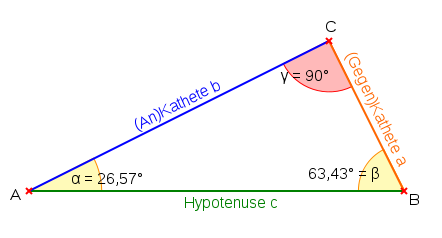
\includegraphics[width=0.6\textwidth,height=.8\textheight,keepaspectratio]{dreieck.png}
	\end{center}
	
	\begin{block}{Cosinusregel}
		\begin{itemize}
			\item $c^2 = a^2 + b^2 - 2 * a * b * \cos \gamma$
			\item $b^2 = a^2 + c^2 - 2 * a * c * \cos \beta$
			\item $a^2 = b^2 + c^2 - 2 * b * c * \cos \alpha$
		\end{itemize}
	\end{block}
\end{frame}

\begin{frame}{Trigonometrie}
	\begin{center}
		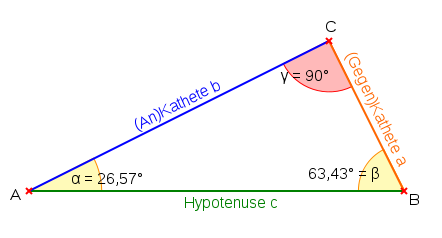
\includegraphics[width=0.6\textwidth,height=.8\textheight,keepaspectratio]{dreieck.png}
	\end{center}
	
	\begin{block}{Sinusregel}
		$\frac{a}{\sin \alpha} = \frac{b}{\sin \beta} = \frac{c}{\sin \gamma} = \frac{a * b * c}{2 * F}$,
		wobei F der Flächeninhalt des Dreiecks ist.
	\end{block}
\end{frame}

\begin{frame}{Trigonometrie}
	\begin{block}{atan2(y, x)}
		\textit{Gegeben:} Punkt $(x,y)$\\ \ \\
		
		\hangindent+20pt \hangafter=1
		\textit{Rückgabewert:} Winkel (in RAD) zwischen der x-Achse und dem Punkt $(x,y)$. Der Wert hat ein \textbf{positives} Vorzeichen, wenn die Drehung \textbf{gegen} den Uhrzeigersinn erfolgt, ansonsten negatives Vorzeichen.\\ \ \\

		Der Wertebereich ist $-\pi < atan2(y, x) \leq \pi$.
	\end{block}
	
	Hinweis: Um von RAD zu DEG zu konvertieren, ist eine Multiplikation mit $\frac{180}{\pi}$ nötig.
\end{frame}

\begin{frame}{Trigonometrie}
	\begin{block}{Winkelberechnung zwischen drei Punkten}
		\textit{Gegeben:} Drei Punkte $a, o, b$\\
		\textit{Gesucht:} $\sphericalangle aob$\\ \ \\

		Formel: $\cos \phi = \left|\frac{\overrightarrow{oa} \cdot \overrightarrow{ob}}{\norm{\overrightarrow{oa}}_2 * \norm{\overrightarrow{ob}}_2}\right|$\\
	\end{block}
	
	\lstset{
		language=C++,
		tabsize=1
	}
	\lstinputlisting[firstline=52, lastline=59]{vectors.cpp}
\end{frame}
